\documentclass[a4paper]{article}

%% Language and font encodings
\usepackage{polski}
\usepackage[polish]{babel}
\usepackage[utf8x]{inputenc}
\usepackage[T1]{fontenc}
\usepackage{pdfpages}
\usepackage{indentfirst}

% Adjust penalties
\brokenpenalty=1000
\clubpenalty=1000
\widowpenalty=1000

%% Sets page size and margins
\usepackage[a4paper]{geometry}

%% Useful packages
\usepackage{amsmath}
\usepackage{graphicx}
\usepackage[colorinlistoftodos]{todonotes}
\usepackage[colorlinks=true, allcolors=blue]{hyperref}

\usepackage{float}

\renewcommand\thesection{\arabic{section}.}
\renewcommand\thesubsection{\arabic{section}.\arabic{subsection}.}
\renewcommand\thesubsubsection{\arabic{section}.\arabic{subsection}.\arabic{subsubsection}.}

\newcommand{\code}{\texttt}

\title{The Project Game}
\author{
Adam Bernat \\
Tomasz Chudzik \\
Marcin Godniak \\
Adrian Sadłocha \\
Michalina Tumialis
}



\begin{document}
\maketitle
\setcounter{secnumdepth}{2}
\setcounter{tocdepth}{2}
\tableofcontents
\newpage

\listoftodos
\newpage

\section{Cel projektu}

Celem jest zaplanowanie oraz~implementacja gry symulującej pracę w środowisku projektowym.
Szczególny nacisk kładziony jest na badanie wpływu zachowań poszczególnych graczy (tj. członków rywalizujących zespołów) na efektywność.

\section{Opis gry}

Gra jest toczona przez dwa rywalizujące zespoły.
Oba zespoły składają się z~wielu graczy oraz~z~jednego wyróżnionego -- lidera zespołu.

Gra jest rozgrywana na prostokątnej planszy, która jest podzielona na trzy strefy: dwie strefy celu (po jednej na każdą drużynę) oraz~na~środkową strefę -- strefę zadań.
Zadania do przedsięwzięćia przez zespoły są reprezentowane przez kawałki.
Są one umieszczane w strefie zadań, z~której to muszą zostać podniesione przez graczy, a następnie zaniesione do strefy celu.
W strefie celu gracz jest w stanie stwierdzić, czy podniesiony kawałek był fałszywką, czy nie.

Każdy gracz przechowuje własny stan gry.
Gracze mogą się ze sobą komunikować, wykazując różne wzorce zachowań.
Prawdziwy stan gry jest przechowywany przez mistrza gra, który jest odpowiedzialny za wygenerowanie planszy oraz~umieszczanie nowych kawałków w strefie zadań.
Wszelka komunikacja pomiędzy mistrzem gry a graczami odbywa się poprzez serwer komunikacyjny.

\section{Słowniczek pojęć}

\begin{itemize}
\item
  Gracz (\emph{player}) - agent grający w grę;
\item
  Mistrz gry (\emph{game master}) - generuje planszę oraz kształt celu, przechowuje rzeczywisty stan gry oraz generuje nowe kawałki;
\item
  Serwer komunikacyjny (\emph{communication server}) - odpowiedzialny za komunikację między graczami, a mistrzem gry;
\item
  Kawałek (\emph{piece}) - token, reprezentujący zasób. Może być fałszywy lub nie;
\item
  Plansza (\emph{board}) - prostokątny obszar, podzielony na kafelki;
\item
  Strefa celu (\emph{goal area}) - część planszy, na której gracze umieszczają kawałki;
\item
  Strefa zadań (\emph{tasks area}) - część planszy, z której gracze podnoszą kawałki;
\item
  Projekt (\emph{project}) - symulowany projekt; ma swój cel, który jest reprezentowany kształtem w strefie celu;
\item
  Cel gry (\emph{game goal}) - odkrycie kształtu projektu poprzez umieszczanie kawałków w strefie celu;
\item
  Zespół (\emph{team}) - grupa współpracujących graczy, dążących do osiągnięcia celu gry;
\item
  Lider (\emph{leader}) - jeden wyrózniony gracz w każdym zespole;
\item
  Gra (\emph{project game}) - gra czasu rzeczywistego, odbywająca się na planszy, gdzie rywalizują dwa zespoły.
\end{itemize}

\section{Reguły gry}

\begin{itemize}
\item
  Nie można wejść w strefę celu przeciwnika;
\item
  Mając kawałek można wejść na pole z innym kawałkiem;
\item
  Gra się kończy, gdy którakolwiek drużyna odkryje wszystkie cele;
\item
  Gracze w obrębie jednego zespołu mogą mieć inne strategie;
\item
  Na jednym polu może znajdować się co najwyżej jeden gracz;
\item
  Odpowiadamy całą planszą przy wymianie informacji;
\item
  Wymiana informacji przebiega w jedną stronę;
\item
  Podczas wymiany informacji, obydwaj gracze tracą czas;
\item
  Jednym z konfigurowalnych ustawień gry jest ``komunikacja pomiędzy zespołami'' (jako \texttt{true}/\texttt{false}). Nazwijmy to roboczo ``flagą komunikacji'';
\item
  Podawanie fałszywych informacji jest zabronione;
\item
  Lider ma obowiązek odpowiadania swojemu zespołowi;
\item
  Lider ma obowiązek odpowiadanie przeciwnemu zespołowi, o ile jest ustawiona ``flaga komunikacji'';
\item
  Jeśli dane pole nie jest celem, to kawałek \emph{nie} znika po odłożeniu. Można (być może warto) go wtedy podnieść;
\item
  Gracz raczej nie powinien zostawiać lipnych kawałków w strefie celu, ale nie jest to formalny wymóg;
\item
  Można przechodzić przez pola z kawałkami i ich nie podnosić;
\item
  Zawsze widzimy pole pod sobą (wraz z odległością do najbliższego kawałka, być może równą 0);
\item
  Podniesienie kawałka zwraca graczowi informację odległość do najbliższego kawałka;
\item
  Cel odkrywamy tylko poprzez położenie kawałka, nie poprzez odkrywanie pól dookoła;
\item
  Kawałek można testować tylko, jeśli aktualnie podniesiony przez gracza, który go chce przetestować;
\item
  Odłożenie kawałka na pole sprawia, że kawałek tam zostaje, niezależnie od tego, czy to cel;
\item
  Znamy tylko pozycje graczy, nie to, czy ``mają w ręku'' kawałek;
\item
  Przy generowaniu planszy, stosujemy symetrię środkową ułożenia celu;
\item
  W przypadku kawałka, który nie jest prawdziwy, przy odkładaniu, nie dostajemy informacji, czy to pole celu, czy też nie;

  \begin{itemize}
  \item
    Tym gracz się dowiaduje, że to nie był prawdziwy kawałek;
  \end{itemize}
\item
  W przypadku prawdziwego kawałka, przy odkładaniu, dostajemy informację, czy to pole celu, czy też nie;
\item
  Mistrz gry może usunąć nieprawdziwy kawałek (o ile nie jest aktualnie podniesiony przez któregoś z graczy). Może też wygenerować nowy, na wolnym polu;

  \begin{itemize}
  \item
    Liczba nieprawdziwych kawałków na planszy jest ograniczona i konfigurowalna;
  \end{itemize}
\item
  Wymiana informacji przechodzi przez mistrza gry;
\item
  Niepoprawny ruch (np. ktoś już stoi na danym polu) nic nie kosztuje;
\item
  Game master zarządza i pilnuje opóźnień dla wszystkich graczy;
\item
  Gra nie jest turowa, jest czas rzeczywistego (z opóźnieniami);
\item
  Do serwera komunikacyjnego łączą się bezpośrednio gracze;
\item
  Wszelka komunikacja jest przetwarzana przez mistrza gry, który odpowiada za pilnowanie legalności ruchów oraz za opóźnienia;
\item
  Gracz dostaje informację o odległości od najbliższego kawałka wchodząc na dane pole, informacja nie jest potem uaktualniana;
\item
  Ruch gracza przebiega następująco: gracz wysyła żądanie do mistrza gry, mistrz gry odsyła odpowiedź, czy akcja może zostać wykonana. Jeśli akcja jest dozwolona, wykonywany jest ruch, po czym mistrz gry (po upływie czasu akcji) wysyła odpowiedź, że czas akcji minął. Wraz z tym komunikatem, mistrz gry przesyła aktualny stan planszy pod graczem, tj. odległość do najbliższego kawałka;
\item
  Po położeniu prawdziwego kawałka na dobry kafelek w strefie celu jest ten kafelek oznaczany jako spełniony cel;
\item
  Mistrz gry tworzy nowe kawałki według dowolnej strategii (z dokładnością do limitu nieprawdziwych kawałków);
\item
  Akcje sprawdzenia położenia wszystkich graczy wraz z odległością do najbliższego kawałka z aktualnej pozycji gracza ma zerowy koszt czasowy;
\item
  Wszystkie inne akcje (łącznie z prośbą o komunikację) mają konfigurowalny, zapewne niezerowy koszt;
\item
  Podczas oczekiwania na odpowiedź na prośbę o komunikację, gracz może wykonywać inne akcje;
\item
  Gracz widzi odległości tylko do kawałków położonych w strefie zadań i strefie celu swojej drużyny;
\item
  Po odłożeniu kawałka w strefie celu, jeśli kawałek był nieprawdziwy, gracz otrzymuje informację, że kawałek nie był prawdziwy. Jeśli kawałek był prawdziwy, to gracz otrzymuje informację, czy to było pole celu, czy nie;
\item
  Początkowe ustawienie graczy jest losowane przez mistrza gry.
\end{itemize}

\section{Możliwe akcje}

Poszczególni aktorzy opisani zostali w słowniku pojęć.
Poniżej przedstawione zostaną możliwe do wykonania przez nich akcje.

\subsubsection{Przypadki użycia}

\begin{figure}[H]
\caption{Przypadki użycia gracza}
\centering
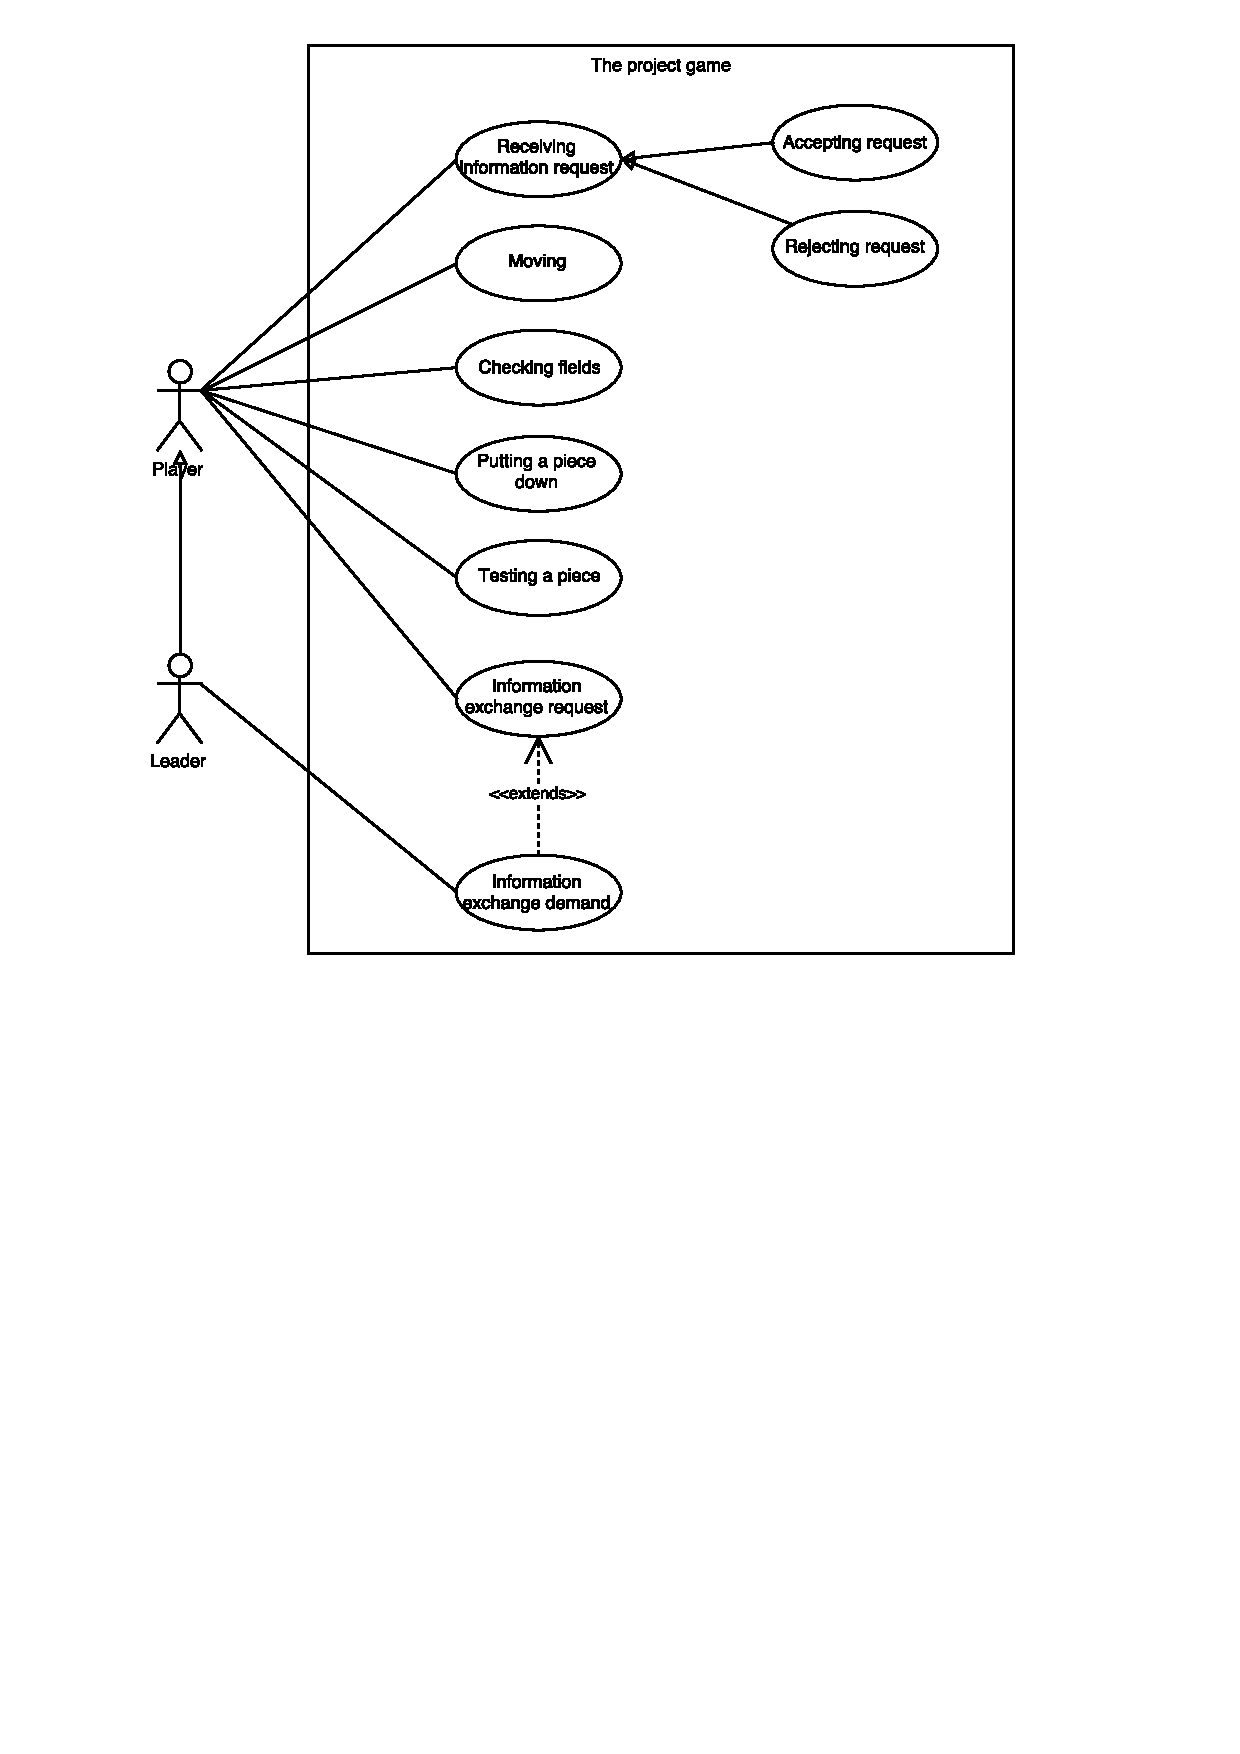
\includegraphics[scale=0.9]{przypadki_uzycia_gracz_lider.pdf}
\end{figure}

Gracz może otrzymać prośbę o wymianę informacji.
Prośba może zostać zaakceptowana lub~odrzucona.
Wyjątkiem jest prośba o wymianę informacji od lidera zespołu -- ta nie może zostać odrzucona.

Gracz może poruszać się w jednym z~czterech kierunków (góra, dół, prawo, lewo).
Nie może jednak wejść na pole celu przeciwnego zespołu.

Gracz ma również do dyspozycji następujące akcje: sprawdzenie pól dookoła, podniesienie kawałka z~aktualnego pola, przetestowanie kawałka (o ile gracz znajduje się w strefie celu).
Ponadto, gracz może wysłać prośbę o wymianę informacji do innego gracza.
W szczególności, może zarządać wymiany informacji od lidera.

\begin{figure}[H]
\caption{Przypadki użycia mistrza gry}
\centering
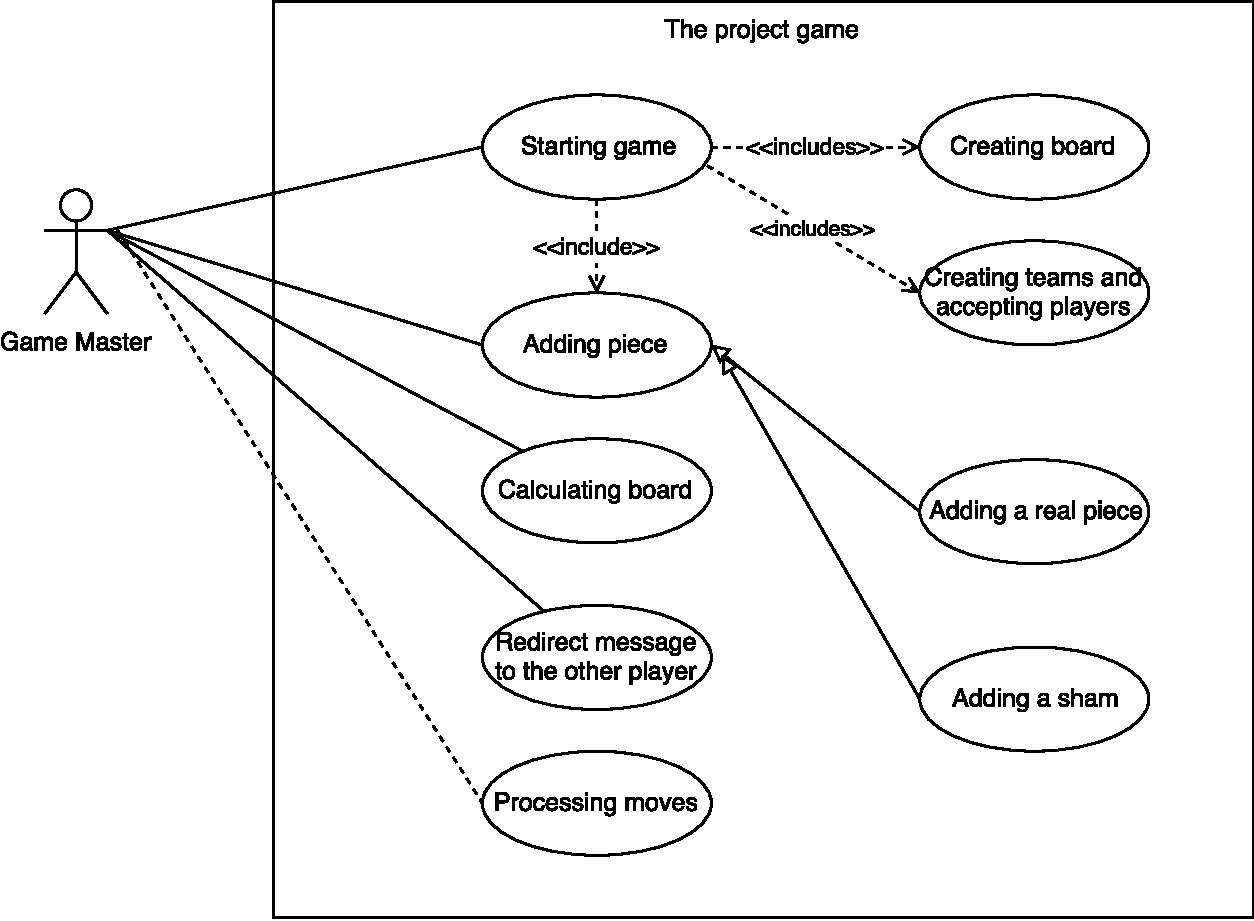
\includegraphics[scale=0.7]{przypadki_uzycia_gm.pdf}
\end{figure}

Mistrz gry rozpoczyna grę, tj. generuje planszę oraz~czeka (i akceptuje) łączących się graczy.
Następnie -- podczas gry -- dodaje kawałki (fałszywe lub nie) do strefy zadań; przelicza odległości do najbliższych kawałków; przekierowuje wiadomości pomiędzy graczami; oraz~przetwarza ruchy graczy.

\begin{figure}[H]
\caption{Przypadki użycia serwera komunikacyjnego}
\centering
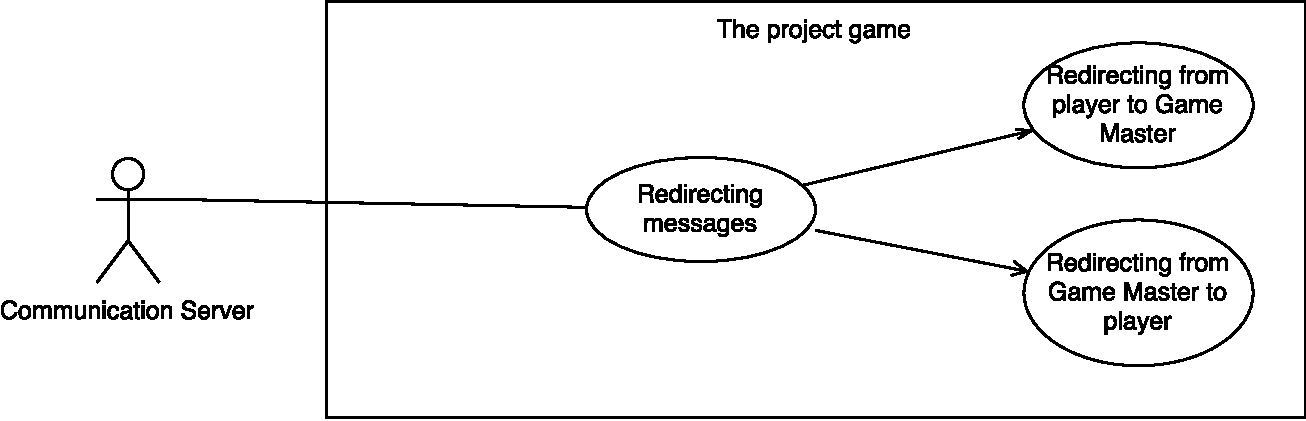
\includegraphics[scale=0.7]{przypadki_uzycia_cs.pdf}
\end{figure}

Serwer komunikacyjny odpowiada za przekierowywanie wiadomości pomiędzy graczami a mistrzem gry.

\section{Możliwości konfguracyjne}
Możliwość konfiguracyjne kontrolują zasady i przebieg rozgrywki, część z nich jest znana wszystkim uczestnikom gry, ale każdy z uczestników posiada również swoje, indywidualne ustawienia. W związku z powyższym,  konfiguracyjne możemy podzielić na trzy grupy, konfiguracja rozgrywki, konfiguracja mistrza gry i konfiguracja gracza.

\subsection{Konfiguracja rozgrywki}
Konfiguracja rozgrywki jest znana każdemu graczowi i mistrzowi gry, zawiera wszelkie dane potrzebne do poprawnego przeprowadzenia rozgrywki, możemy wydzielić następujące dane:
  \begin{itemize}
  \item
    Koszt czasowy każdego z ruchów.
  \item
    Rozmiar planszy, czyli rozmiar strefy celu i strefy zadań.
  \item 
    Liczbę graczy w każdej z drużyn.
  \item 
    Informacje który z graczy jest liderem drużyny.
  \end{itemize}

\subsection{Konfiguracja mistrza gry}
Mistrz gry posiada konfiguracje, którymi nie dzieli się z graczami biorącymi udział w rozgrywce:
  \begin{itemize}
  \item
    Ilość i położenie pól w strefie celu.
  \item
    Maksymalną ilość kawałków jednocześnie znajdujących się na planszy.
  \item 
    Procentowy udział fałszywek w ramach wszystkich kawałków.
  \end{itemize}
  
\subsection{Konfiguracja gracza}
Każdy z graczy posiada konfiguracje, która umożliwia sterowaniem zachowaniem podczas rozgrywki, między innymi:
  \begin{itemize}
  \item
    identyfikator drużyny, do której należy. 
  \item
    Strategia akceptacji próśb o udzielenie informacji.
  \item
    Poziom agresywności w szukaniu kawałków.
  \item
    Ustawienia strategii dotyczącej sprawdzania kawałków. 
  \end{itemize}
 

\section{Uruchamianie aplikacji}
Serwer komunikacyjny, mistrz gry i każdy z graczy stanowią osobne programy, każdy z nich może znajdować się na osobnej maszynie. Podczas uruchamiania programu gracza należy przekazać namiary na serwer komunikacyjny, ścieżkę do pliku z ustawieniami rozgrywki i do pliku z konfiguracją gracza:

./Gracz --SC=192.168.1.20:9876 ./KonfiguracjaRozgrywki.xml ./KonfiguracjaGracza.xml

Aplikacje mistrza gry uruchamiamy w bardzo podobny sposób, ale zamiast ścieżkę do pliku z ustawianiami gracza przekazujemy ścieżkę do pliku z ustawieniami mistrza gry:

./Mistrz --SC=192.168.1.20:9876 ./KonfiguracjaRozgrywki.xml ./KonfiguracjaMistrzaGry.xml

Musimy również uruchomić serwer komunikacyjny, jedyny parametr, który musimy przekazać to port, na którym będzie nasłuchiwał nadchodzącej komunikacji:

./SerwerKominukacyjny --PORT=9876

Kolejność uruchamiania aplikacji nie ma znaczenia, jednak najlepiej rozpocząć proces do uruchomienia serwera komunikacyjnego, w ten sposób będziemy znali port, na którym nasłuchuje i w razie problemów z zajęciem danego portu będziemy mieć okazje od razu zareagować. Następnie najlepiej uruchomić mistrza gry, jeżeli uruchomimy go przed aplikacjami gracza będzie on mógł od razu odpowiedzieć na prośby przyłączenia do gry.

Po zakończeniu rozgrywki, każda z aplikacji wypisuje podsumowanie, gry po czym kończy działanie.

\section{Wymagania niefunkcjonalne}
System ma za zadanie umożliwić sprawny przebieg rozgrywki dla dwóch drużyn rozmiaru do 20 graczy w każdej.
W związku z tym, aplikacje serwera komunikacyjnego i mistrza gry, powinny być zoptymalizowane pod względem wydajności obliczeniowej i wykorzystania łącza sieciowego, tak aby mogły być uruchomione w warunkach laboratorium wydziałowego. 

W razie utraty łączności pomiędzy uczestnikami gry a serwerem komunikacyjnym, aplikacje aktywnie próbują odzyskać łączność przez czas nie krótszy niż 30 minut. Szczegółowy opis procesu znajduje się w rozdziale 13. Opis sytuacji wyjątkowych.

Każdy z programów powinien dostarczać po podaniu parametru --help, krótki opis funkcjonalności wraz z opisem procesu uruchomienia.

Programy graczy i mistrza gry, potrafią zaprezentować użytkownikowi aktualny widziany przez nich stan gry. 
\section{Opis architektury}

\subsection{Diagram klas}
\newpage
\begin{figure}[H]
\caption{Diagram klas}
\centering
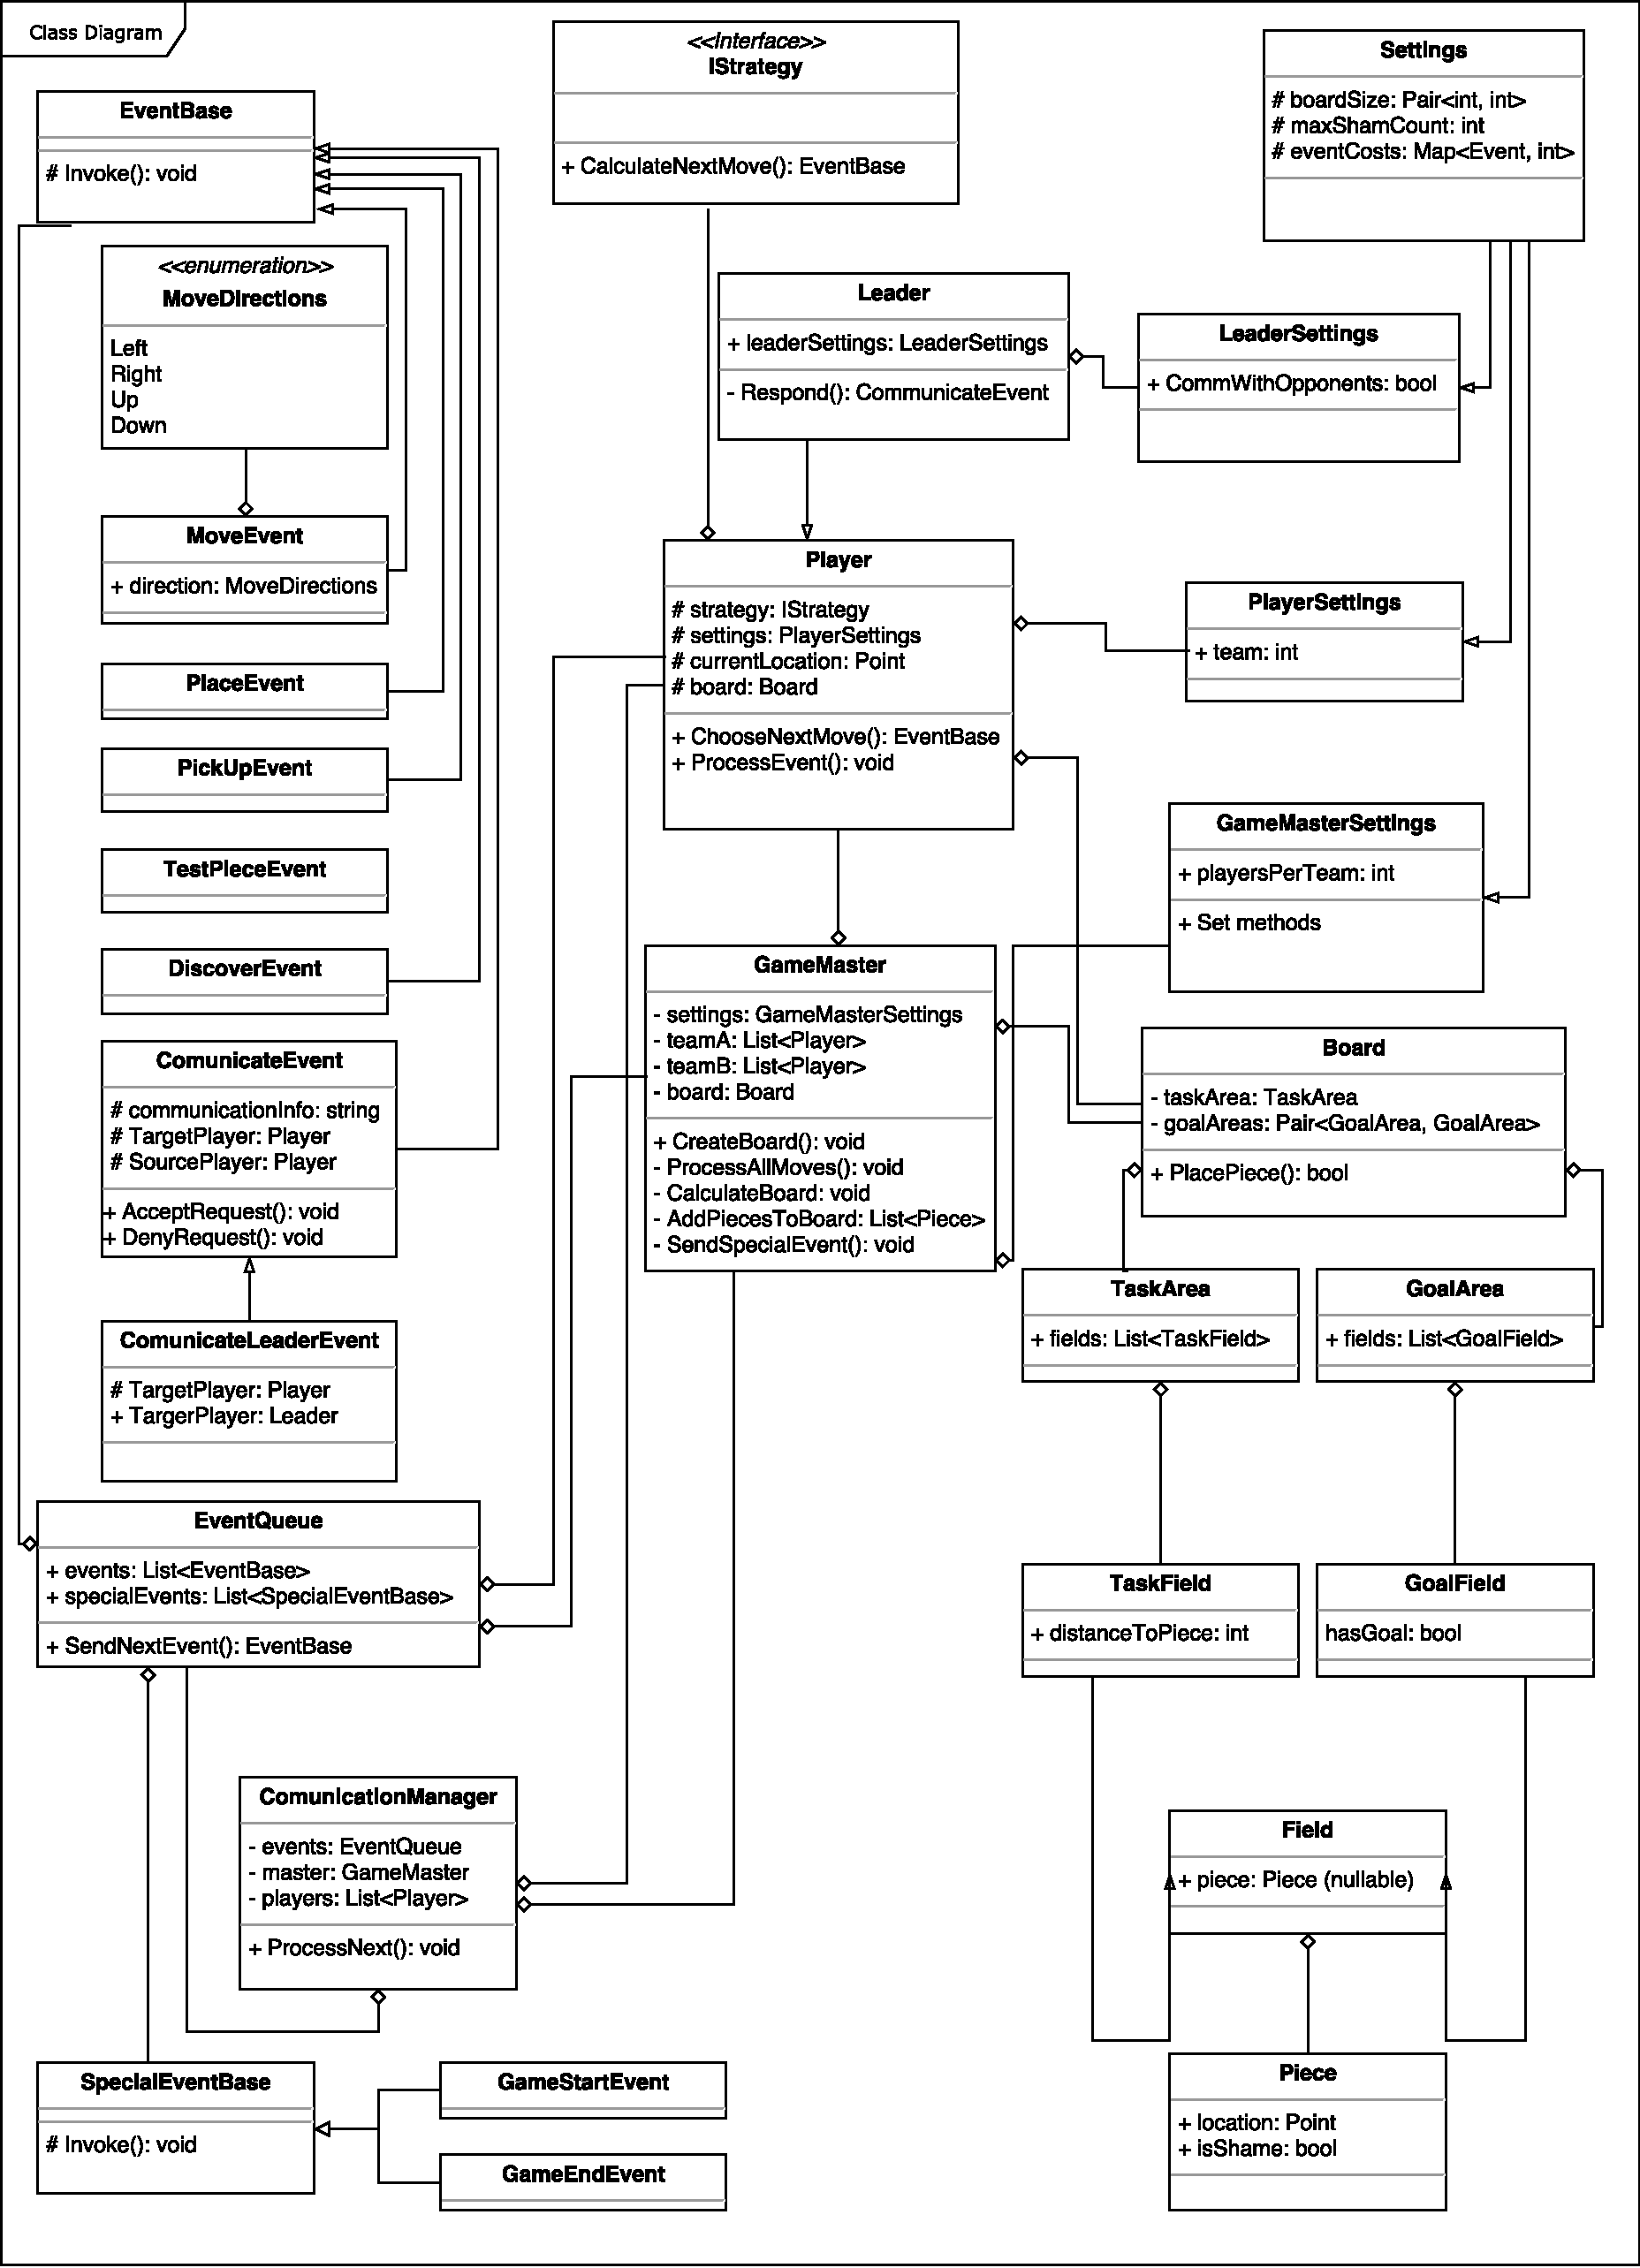
\includegraphics[scale=0.47]{diagram_klas.pdf}
\end{figure}

Klasa gracza zawiera pole strategii, odpowiedzialnej za wyliczanie kolejnych ruchów.
Ponadto, klasa przechowuje pole ustawień (numer zespołu, rozmiar planszy, maksymalna liczba dopuszczalnych fałszywek oraz~mapę kosztów poszczególnych ruchów).
Gracz przechowuje również swoja aktualną pozycję na planszy oraz~referencję do obiektu planszy.
Gracz może wybrać swój następny ruch oraz~może przetwarzać nadchodzące wydarzenia.
Lider jest specjalnym rodzajem gracza, mającym dodatkowe ustawienie -- czy musi się komunikować z~przeciwną drużyną, czy nie.

\hfill 

W grze występują następujące wydarzenia:
\begin{itemize}
    \item \code{MoveEvent} -- zawiera kierunek ruchu (lewo, prawo, góra, dół);
    \item \code{PickUpEvent} oraz~\code{PlaceEvent} -- wydarzenia mające miejsce, gdy gracz kolejno podnosi lub~odkłada kawałek;
    \item \code{TestPieceEvent} -- akcja sprawdzania przez gracza, czy kawałek jest fałszywką, czy nie;
    \item \code{DiscoverEvent} -- sprawdzenie przez gracza pól dookoła;
    \item \code{CommunicateEvent} -- prośba o wymianę informacji pomiędzy dwoma graczami (prośba o wymianę informacji może zostać zaakceptowana lub odrzucona; jedynie lider ma obowiązek odpowiadania na prośby);
\end{itemize}

Wydarzenia są umieszczanie w kolejce \code{(EventQueue}), która zawiera przedstawione wyżej wydarzenia oraz~dwa specjalne: \code{GameStartEvent} tudzież~\code{GameEndEvent}.

\hfill

Mistrz gry jest klasą odpowiedzalną za stworzenie planszy, przeliczanie stanu gry, dodawania kawałków do planszy, przetwarzenie wszytkich ruchów graczy oraz~za wysyłanie specjalnych wydarzeń, takich jak informacja o początku lub końcu gry.
Ta klasa zawiera referencje do obu zespołów, planszy; przetrzumuje rownież obiekt ustawień z~informacjami takimi jak liczba graczy w drużynie.

Komunikacja pomiędzy graczami a mistrzem gry odbywa się za~pośrednictwem serwera komunikacyjnego.
Przetrzumuje on listę wydarzeń, graczy oraz~referencję na mistrza gry.

Podstawowa klasa ustawień (Settings) zawiera informacje o rozmiarach planszy (za pomocą pary liczb całkowitoliczbowych zdefiniowana jest szerokość i~wysokość), maksymalnej liczbie fałszywek.
Ponadto, przechowuje mapę kosztów poszczególnych akcji.

Klasa planszy zawiera trzy strefy: jedną strefę zadań oraz~dwie strefy celu.
Strefa zadań przechowuje pola, na których mogą znajdować się kawałki.
Pola te zawierają odległość do najbliższego kawałka.
Każda strefu celu zaś przechowuje pola, które mogą być częścią celu.
Odkrywa się je, poprzez odkładanie na nich prawdziwych kawałków.
Pola celu zawierają zmienną typu logicznego, która określa, czy jest to część zadania.

Klasa kawałków przechowuje swoją lokalizację na planszy oraz~pole logiczne informujące o~prawdziwości kawałka.

\section{Diagram aktywności}
\begin{figure}[H]
\caption{Diagram aktywności}
\centering
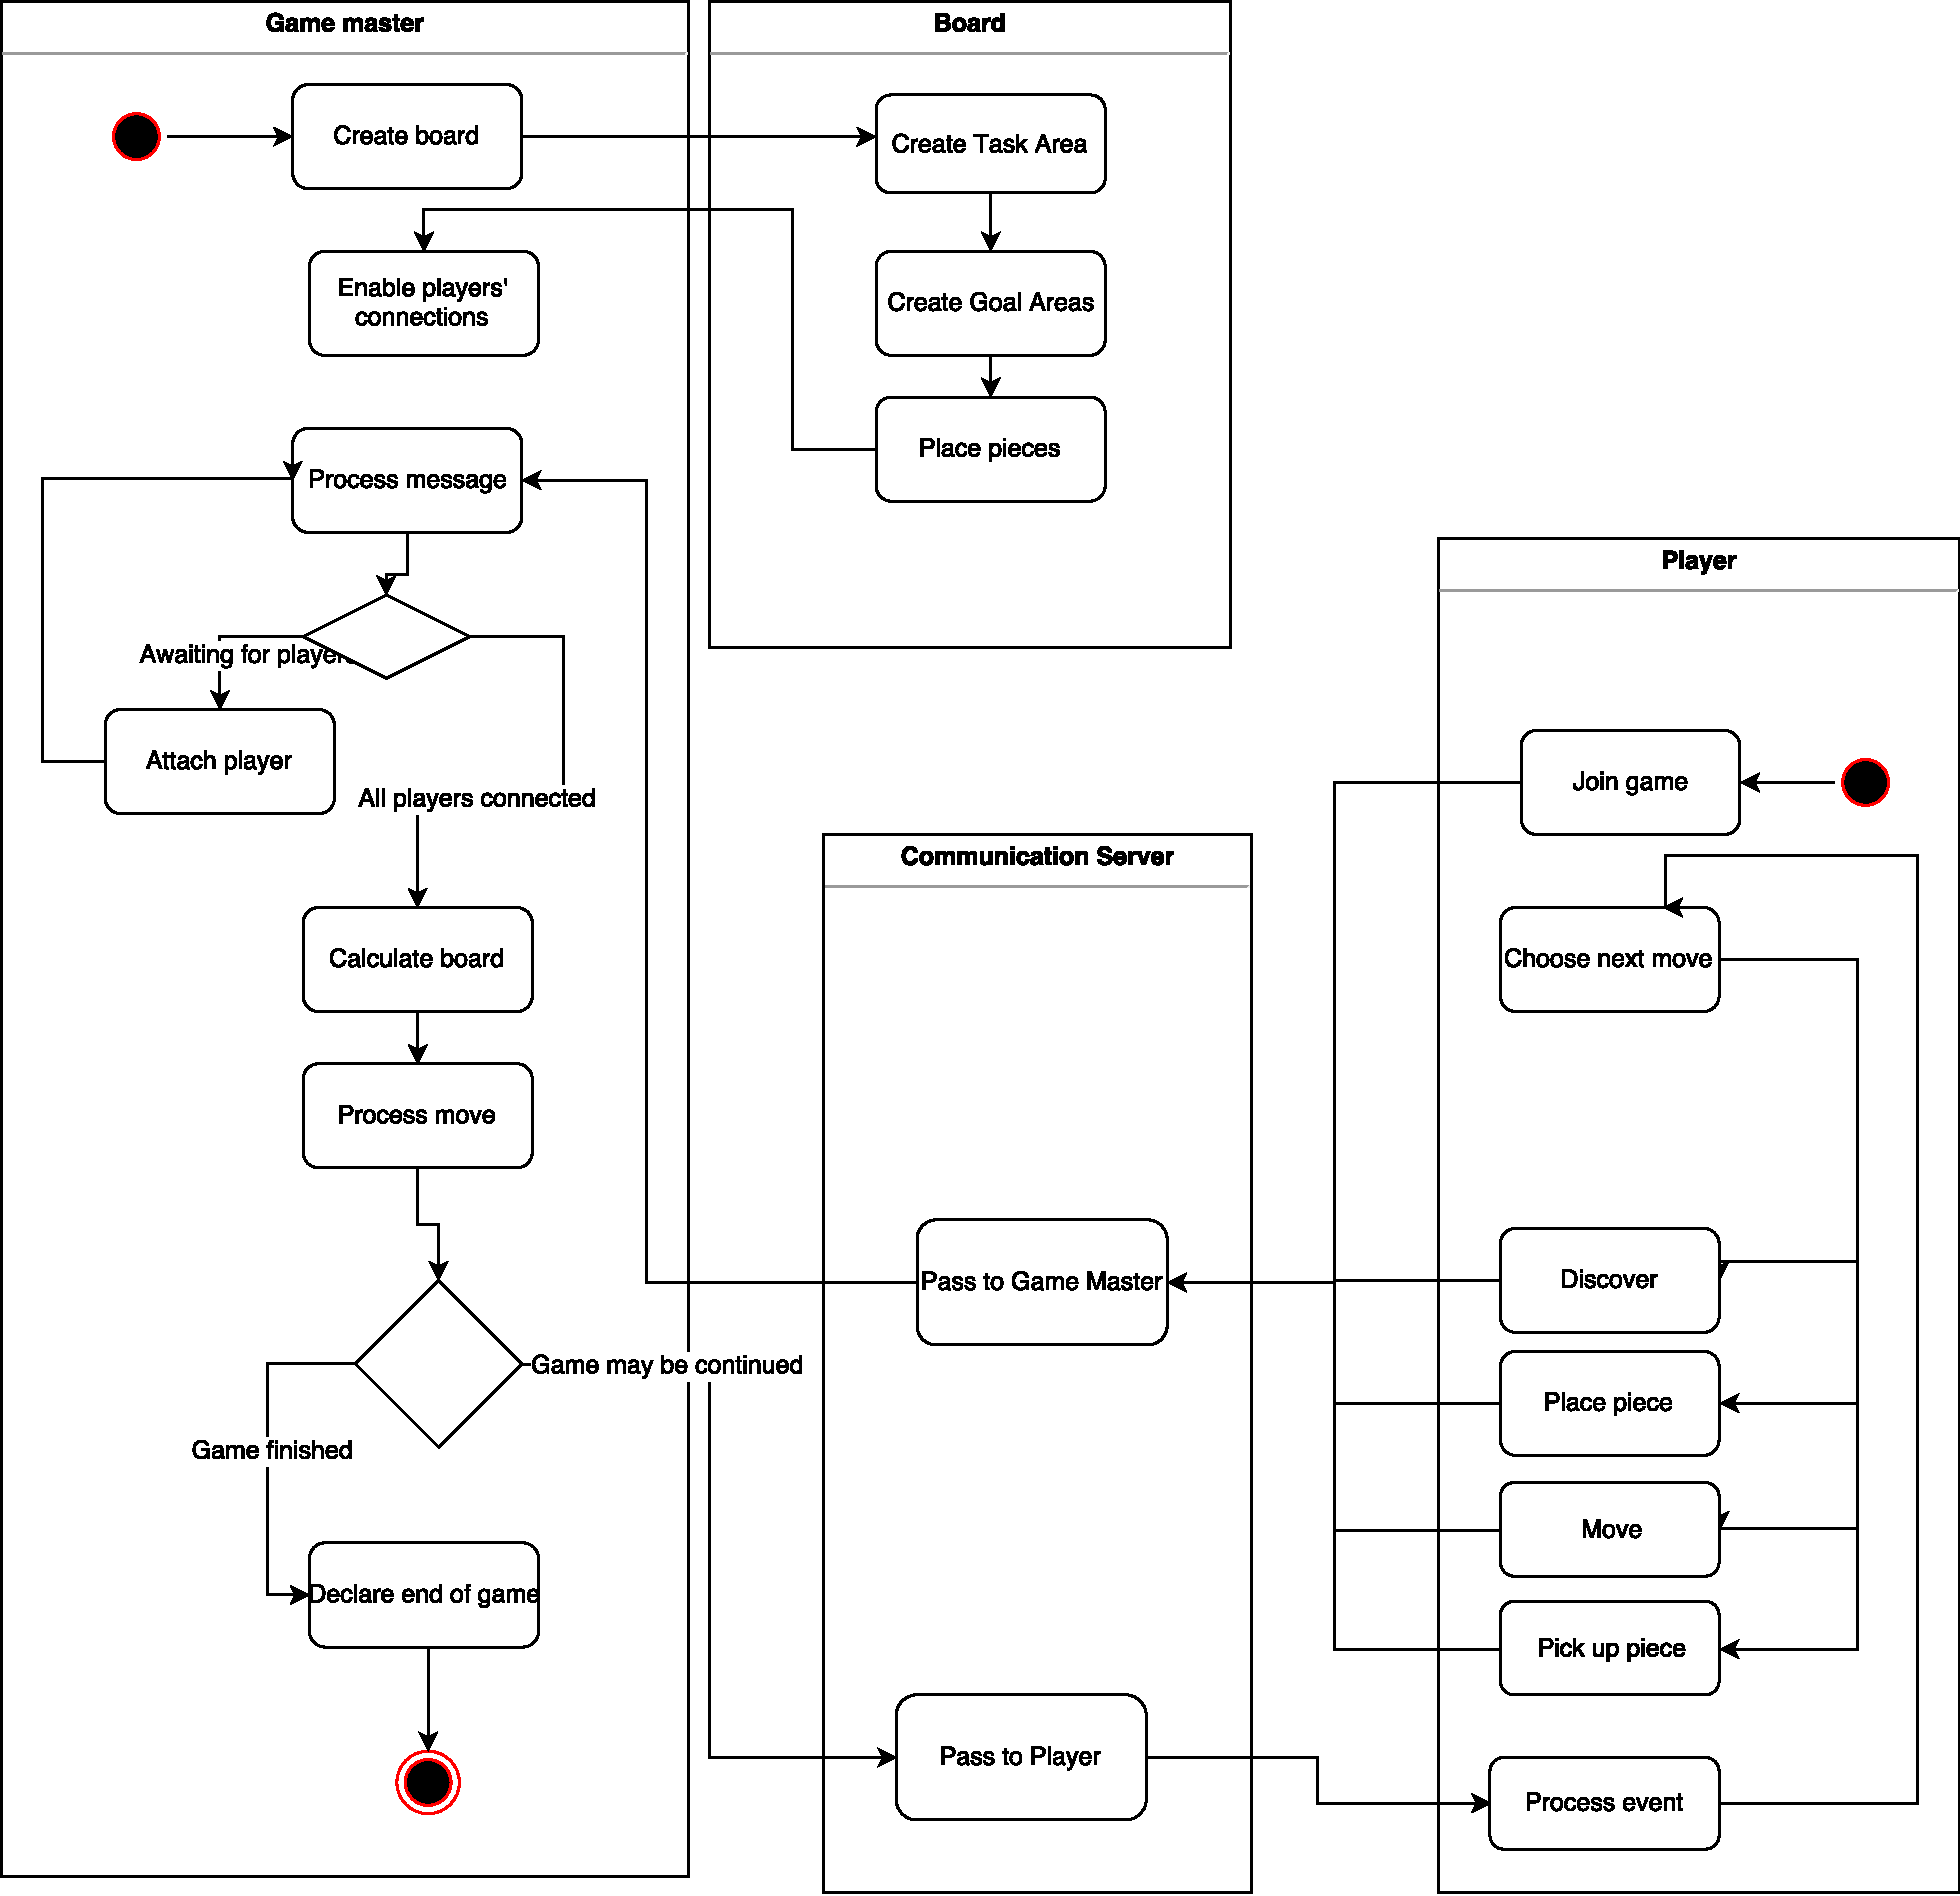
\includegraphics[scale=0.5]{diagram_aktywnosci.pdf}
\end{figure}
Po rozpoczęciu gry, mistrz gry tworzy planszę: strefę zadań; strefy celów; umieszcza kawałki.
Następnie czeka aż gracze się połączą.

Po podłączeniu wszystkich graczy, mistrz gry utrzymuje stan planszy oraz~obsługuje ruchy graczy.
Kiedy gra zostanie zakończona, informuje graczy o końciu rozgrywki.

Gracze mogą dołączyć do gry i~wykonywać ruchy: odkrywanie pól dookoła; ruch w jednym z~czterech kierunków; podniesienie lub odłożenie kawałka.
Ruchy są przekazywane do mistrza gry (i odpowiedzi są przekazywane z~powrotem do gracza) za~pośrednictwem serwera komunikacyjnego.


\section{Diagram stanów}
\begin{figure}[H]
\caption{Diagram stanów gracza}
\centering
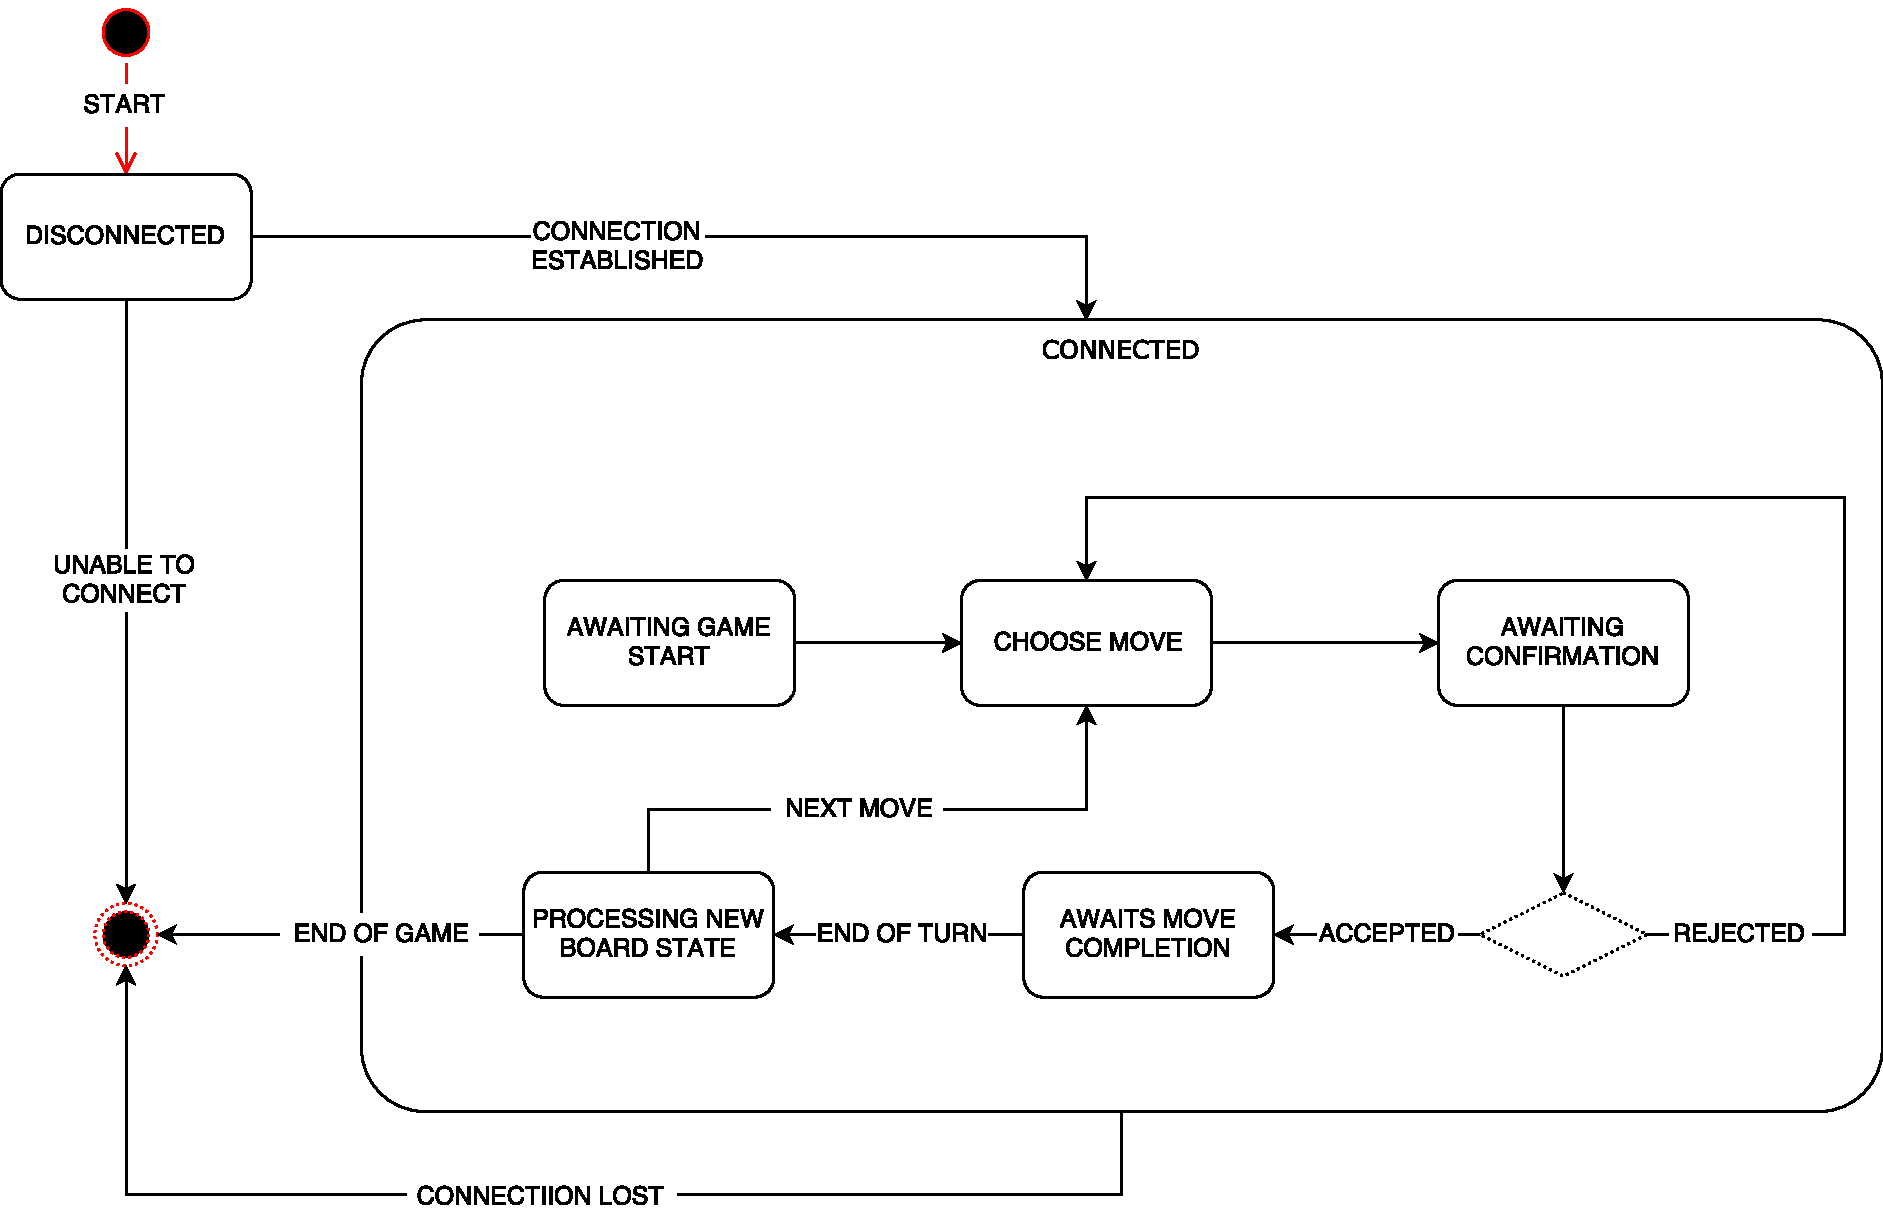
\includegraphics[scale=0.5]{state_diagram_player.pdf}
\end{figure}

Na początku, gracz jest w stanie rozłączonym i~próbuje połączyć się z~grą.
Jeśli się to nie uda, kończy działanie.

Jeśli jednak połączenie zostanie nawiązane, to gracz oczekuje na rozpoczęcie gry.
Po rozpoczęciu gry, gracz -- w pętli -- wykonuje ruch, oczekuje odpowiedzi, czeka na zakończenie ruchu, przetwarza nowy stan gry.
Jeśli ruch zostanie odrzucony przez mistrza gry, gracz od razu próbuje wykonać kolejny ruch.

Jeśli w którymś momencie gracz otrzyma wiadomość o zakończeniu gry (lub utraci połączenie), kończy działanie.

\section{Protokół komunikacyjny}

\subsection{Rozpoczęcie gry}
\begin{figure}[H]
\caption{Diagram sekwencji: rozpoczęcie gry}
\centering
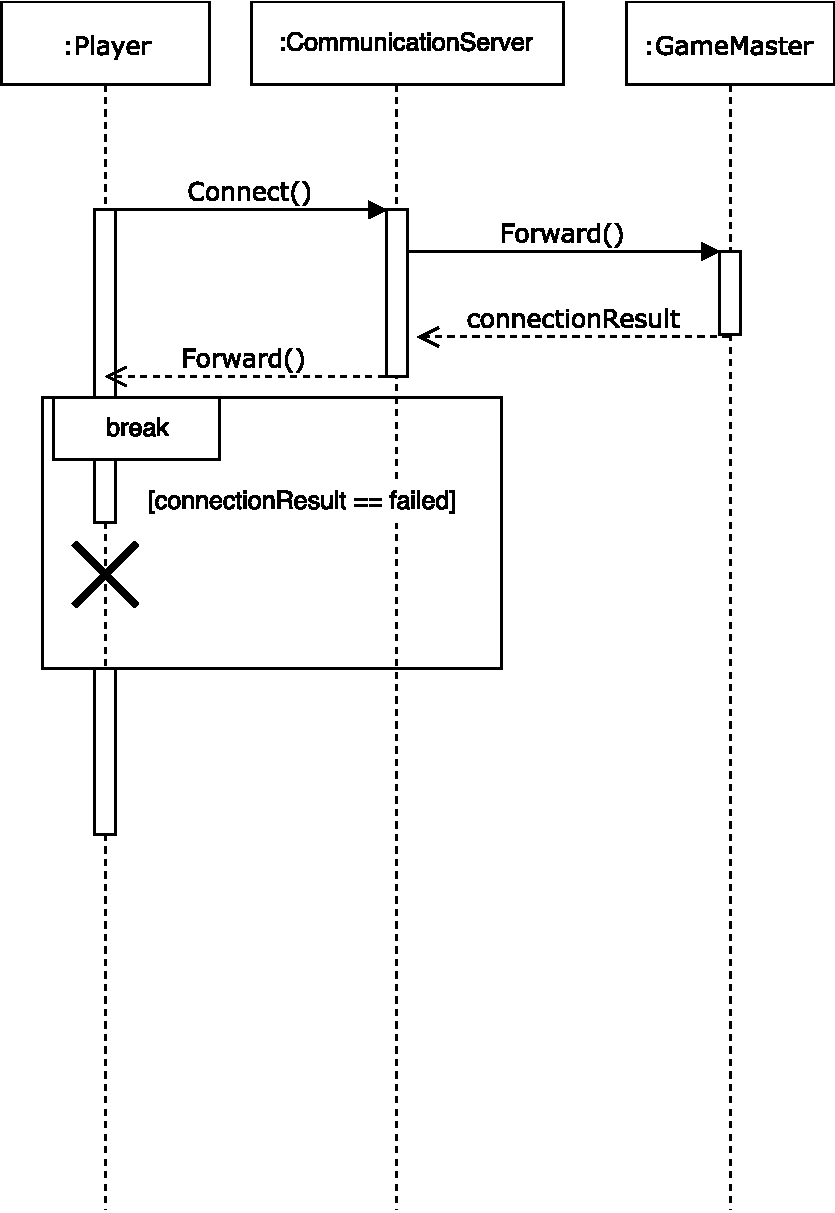
\includegraphics[scale=0.8]{sekwencje1.pdf}
\end{figure}

Najpierw gracz wywołuje metodę \code{Connect()} i~czeka na odpowiedź od serwera komunikacyjnego, który to przekierowuje zapytanie do mistrza gry i~czeka na odpowiedź, którą przekazuje do gracza.
Jeśli gracz zostanie dodany do gry, bierze udział w grze.
W przeciwnym przypadku kończy działanie.

\subsection{Komunikacja między graczem i mistrzem gry}
\begin{figure}[H]
\caption{Diagram sekwencji: gracz - mistrzy gry}
\centering
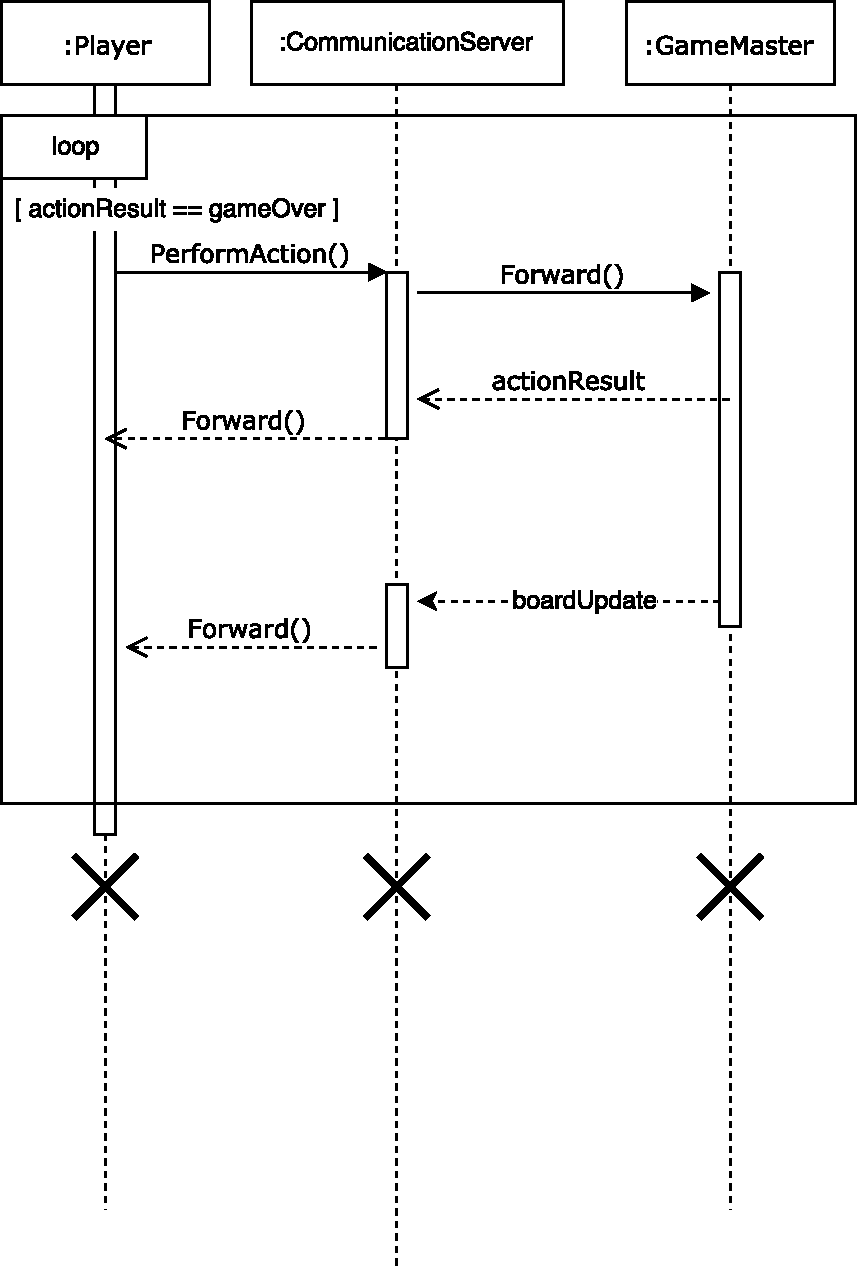
\includegraphics[scale=0.8]{sekwencje2.pdf}
\end{figure}

Gracz wykonuje ruchy w pętli, która kończy się, gdy dostanie odpowiedź (z serwera komunikacyjnego) z~komunikatem ,,koniec gry''.
Serwer komunikacyjny dostaje informacje o ruchach wykonywanych przez graczy i~przekazuje je do mistrza gry.
Następnie czeka na odpowiedź, którą przekazuje do gracza.
Ponadto, otrzymuje informacje o komunikatach od mistrza gry, które przekazuje graczom.

\subsection{Komunikacja między graczami}
\begin{figure}[H]
\caption{Diagram sekwencji: gracz - gracz}
\centering
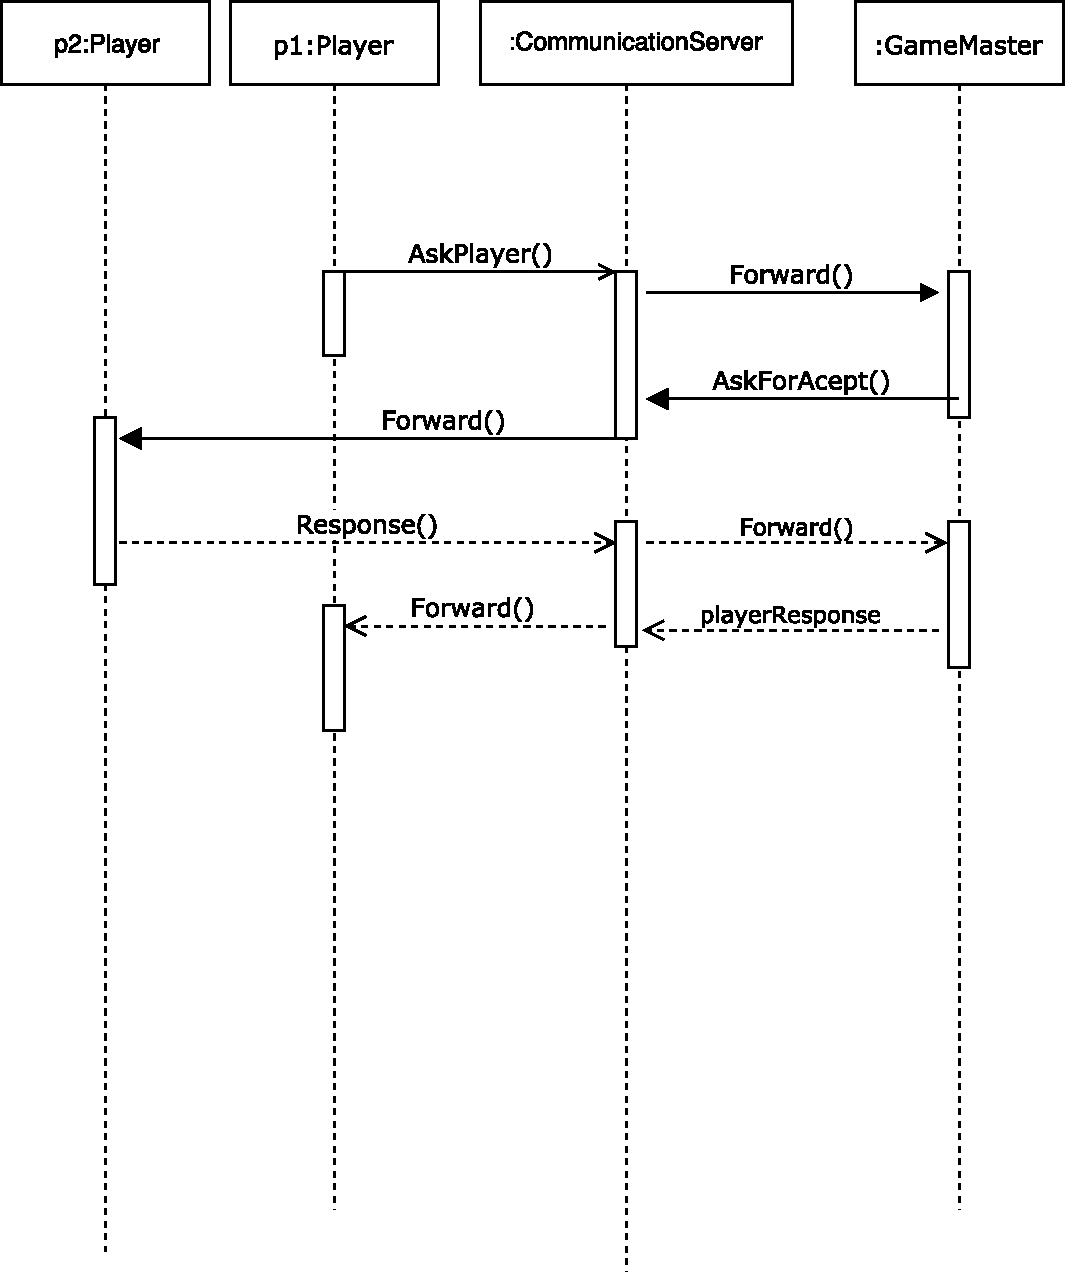
\includegraphics[scale=0.8]{sekwencje3.pdf}
\end{figure}

Komunikacja pomiędzy graczami odbywa się za~pośrednictwem serwera komunikacyjnego i~mistrza gry.

Kiedy gracz \code{p1} chce skomunikować się z~graczem \code{p2}, najpierw wysyła wiadomość do serwera komunikacyjnego.
Serwer komunikacyjny przekazuje zapytanie do mistrza gry, który następnie decyduje, czy taki ruch jest możliwy w danym momencie.
Jeśli tak, to mistrz gry wysyła zapytanie (zawierające pole nadawcy, czyli gracza \code{p1}) do \code{p2}.
Po otrzymaniu tej wiadomości (ponownie: za~pośrednictwem serwera komunikacyjnego), gracz \code{p2} decyduje o odpowiedzi (akceptacji lub odrzuceniu) i~wysyła ją. Odpowiedź wędruje przez serwer komunikacyjny do mistrza gry, ponownie do serwera komunikacyjnego, aż trafi do gracza \code{p1}.

\subsection{Struktura wiadomości}

Wiadomości są przesyłane w formacie JSON.
W tym dokumencie, dla czytelności, używamy uproszczonego zapisu, w którym słownik jest reprezentowany przez wcięcie w kodzie.
Przykład w~JSON-ie:

\begin{verbatim}
{
    "var1": 5,
    "var2":
        [
            1,
            2,
            3
        ],
    "var3":
        {
            "var3_a": "a",
            "var3_b": "b",
            "var3_c": "c",
        }
}
\end{verbatim}

Ta sama wiadomość w uproszczonym zapisie:

\begin{verbatim}
- var1: 5
- var2:
    - 1
    - 2
    - 3
- var3:
    - var3_a: "a"
    - var3_b: "b"
    - var3_c: "c"
\end{verbatim}

Wszystkie wiadomości muszą mieć pole \code{referenceId} (które jest typu całkowitoliczbowego).
Mistrz gry musi dołączać \code{referenceId} w odpowiedziach.
Ten mechanizm pozwala graczom na dopasowanie poszczególnych odpowiedzi do zapytania, którego ona dotyczy.

Wartość pola \code{referenceId} jest arbitralnie ustalana przez każdego gracza.

\subsubsection{Struktura planszy}

Plansza jest dwuwymiarową tablicą, gdzie pierwszy indeks wskazuje na wiersz, zaś drugi na kolumnę.

\subsubsection{Wiadomości od mistrza gry}

\paragraph{Początek gry}
\hfill
\hfill

Do: wszystkich graczy

Struktura:

\begin{verbatim}
- type: "gameStart"
- body:
    - position_x: <int>
    - position_y: <int>
    - pieceDistance: <int>
\end{verbatim}

\paragraph{Koniec gry}
\hfill

Do: wszystkich graczy

Struktura:

\begin{verbatim}
- type: "gameEnd"
\end{verbatim}

\paragraph{Prośba o komunikację pomiędzy graczami}
\hfill

Struktura:

\begin{verbatim}
- type: "communicationRequest"
- body:
    - playerId: <int>
    - mustAccept: <bool>
\end{verbatim}

Uwaga: pole \code{mustAccept} musi być ustawione według tego, czy żądanie zostało wysłane przez~lidera.

Odpowiedź:

\begin{verbatim}
- type: "communicationRequest"
- body:
    - board: <Board>
\end{verbatim}

\subsubsection{Wiadomości od graczy}

\paragraph{Dołączenie do gry}
\hfill

Struktura:

\begin{verbatim}
- type: "join"
- body:
    - teamId: <int>
\end{verbatim}

Odpowiedź (w przypadku sukcesu):

\begin{verbatim}
- type: "join"
- body:
    - success: True
    - playerId: <int>
    - boardWidth: <int>
    - boardHeight: <int>
    - goalAreaHeight: <int>
    - upperGoalAreaTeamId: <int>
    - maxShamCount: <int>
    - eventCosts: Map<Event, int>
\end{verbatim}

Odpowiedź (w przypadku niepowodzenia):

\begin{verbatim}
- type: "join"
- body:
    - success: False
\end{verbatim}

\paragraph{Ruch w jednym z czterech kierunków}
\hfill

Struktura:

\begin{verbatim}
- type: "move"
- body:
    - direction: <int>
\end{verbatim}

Gdzie \code{direction} jest typu \code{enum}.

Odpowiedź (success):

\begin{verbatim}
- type: "move"
- body:
    - success: True
    - pieceDistance: <int>
\end{verbatim}

Odpowiedź (failure):

\begin{verbatim}
- type: "move"
- body:
    - success: False
    - pieceDistance: <int>
\end{verbatim}

\paragraph{Przetestowanie kawałka}
\hfill

Struktura:

\begin{verbatim}
- type: "test"
\end{verbatim}

Odpowiedź:

\begin{verbatim}
- type: "test"
- body:
    - isSham: <bool>
\end{verbatim}

\paragraph{Odłożenie kawałka}
\hfill

Struktura:

\begin{verbatim}
- type: "place"
\end{verbatim}

Odpowiedź:

\begin{verbatim}
- type: "place"
- body:
    - success: <bool>
\end{verbatim}

\paragraph{Podniesienie kawałka}
\hfill

Struktura:

\begin{verbatim}
- type: "pickUp"
\end{verbatim}

Odpowiedź:

\begin{verbatim}
- type: "place"
- body:
    - success: <bool>
\end{verbatim}

\paragraph{Odkrywanie pól dookoła}
\hfill

Struktura:

\begin{verbatim}
- type: "discover"
\end{verbatim}

Odpowiedź:

\begin{verbatim}
- type: "discover"
- body:
    - discovered: <tuple of 9 nullable ints>
\end{verbatim}

\paragraph{Prośba o komunikację pomiędzy graczami}
\hfill

Struktura:

\begin{verbatim}
- type: "communicationRequest"
- body:
    - targetPlayer: <int>
\end{verbatim}

Odpowiedź (w przypadku akceptacji):

\begin{verbatim}
- type: "communicationRequest"
- body:
    - success: False
    - board: <Board>
\end{verbatim}

Odpowiedź (w przypadku odmowy):

\begin{verbatim}
- type: "communicationRequest"
- body:
    - success: False
\end{verbatim}

\section{Opis sytuacji wyjątkowych}

\subsection{Utrata łączności z graczem}
\todo{Utrata łączności z graczem}

\subsection{Utrata łączności z serwerem komunikacyjnym}
\todo{Utrata łączności z serwerem komunikacyjnym}

\subsection{Utrata łączności z mistrzem gry}
\todo{Utrata łączności z mistrzem gry}

\end{document}
